\documentclass[conference]{IEEEtran}
\usepackage{float}
\IEEEoverridecommandlockouts

\usepackage{amsmath,amssymb,amsfonts}
\usepackage{graphicx}
\usepackage{booktabs}
\usepackage{tikz}
\usetikzlibrary{shapes.geometric,arrows.meta,positioning,fit}
\usepackage{xcolor}
\usepackage{url}
\usepackage{cite}
\usepackage{hyperref}
\usepackage{placeins} % \FloatBarrier -- keeps floats from drifting past a section

\hypersetup{
    colorlinks=true,
    linkcolor=blue,
    citecolor=blue,
    urlcolor=blue
}

% --- Float packing: allow more/larger floats per page so the
% --- full-width figures do not spill onto extra pages.
\renewcommand{\topfraction}{0.95}
\renewcommand{\bottomfraction}{0.95}
\renewcommand{\textfraction}{0.05}
\renewcommand{\floatpagefraction}{0.80}
\renewcommand{\dbltopfraction}{0.95}
\renewcommand{\dblfloatpagefraction}{0.80}
\setcounter{topnumber}{4}
\setcounter{bottomnumber}{3}
\setcounter{totalnumber}{6}
\setcounter{dbltopnumber}{4}

\begin{document}

\title{Hybrid CNN-LSTM Model for Short-Term Solar Power Forecasting with Anomaly-Aware Preprocessing}

\author{
\IEEEauthorblockN{Tushar Basak}
\IEEEauthorblockA{\textit{Department of Electronics \& Communication Engineering} \\
\textit{Faculty of Technology, University of Delhi}\\
Delhi 110007, India \\
tusharbasak555@ece.du.ac.in}
\and
\IEEEauthorblockN{Varun Saxena}
\IEEEauthorblockA{\textit{Department of Electronics \& Communication Engineering} \\
\textit{Faculty of Technology, University of Delhi}\\
Delhi 110007, India \\
varunsaxena@fot.du.ac.in}
}

\maketitle

\begin{abstract}
Accurate ultra-short-term photovoltaic (PV) power forecasting depends not only on forecasting architecture but also on the quality of plant telemetry. This paper investigates an anomaly-aware preprocessing pipeline for 30-minute-ahead PV power forecasting. Using a one-year, 5-minute-resolution NREL dataset from a 70~MW utility-scale PV site, we synthetically inject three classes of telemetry corruption -- daytime dropouts, spike anomalies, and short-duration offset faults -- across $\sim$2\% of observations. An Isolation Forest identifies anomalous observations, which are reconstructed through local linear interpolation. To isolate the contribution of preprocessing from that of detection quality, we evaluate four parallel data conditions: a never-corrupted \emph{pristine} reference (the performance ceiling), \emph{raw corrupted} telemetry, telemetry cleaned by the unsupervised \emph{Isolation Forest} detector (the proposed pipeline), and telemetry cleaned using \emph{oracle} ground-truth corruption labels. The detector achieves 72.21\% recall and 57.48\% precision. All deep learning results are reported as mean $\pm$ standard deviation across 5 random seeds, with paired $t$-tests, a Holm--Bonferroni correction for multiple comparisons, and a Two One-Sided Tests (TOST) equivalence analysis used to validate every comparative claim. The proposed CNN--LSTM achieves RMSE $= 3.57 \pm 0.04$~MW, MAE $= 1.64 \pm 0.08$~MW, and $R^2 = 0.949 \pm 0.001$. Paired tests against the pristine ceiling ($3.58 \pm 0.06$~MW) and the oracle-cleaned condition ($3.58 \pm 0.05$~MW) show no significant difference (Holm-adjusted $p = 1.000$ for both), and a TOST equivalence test confirms the proposed model is statistically indistinguishable from the pristine ceiling within a $\pm 0.10$~MW practical-equivalence margin ($p \approx 0.05$). Against the raw-corrupted ablation ($3.89 \pm 0.11$~MW), cleaning yields an 8.2\% mean RMSE reduction. The proposed model achieves a lower RMSE than a plain LSTM baseline in every one of 5 paired seeds ($3.77 \pm 0.11$~MW; raw paired $t=-3.89$, $p=0.018$), though after Holm--Bonferroni correction for the three pairwise comparisons performed in this study this difference does not reach the conventional 0.05 significance threshold (adjusted $p = 0.053$) and is reported as a consistent, but not conclusively confirmed, architectural advantage. Both deep models outperform persistence (4.93~MW) and a diurnal-lag autoregressive baseline (4.83~MW) by a wide margin.
\end{abstract}

\begin{IEEEkeywords}
Anomaly detection, anomaly-aware preprocessing, CNN--LSTM, Isolation Forest, photovoltaic power forecasting, sensor fault detection, short-term forecasting, time-series imputation, equivalence testing.
\end{IEEEkeywords}

% =================================================================
\section*{Nomenclature}
\addcontentsline{toc}{section}{Nomenclature}

\noindent
\begin{IEEEdescription}[\IEEEsetlabelwidth{SCADA}]
\item[ADC] Analog-to-Digital Converter
\item[CNN] Convolutional Neural Network
\item[DPV] Distributed Photovoltaic
\item[GHI] Global Horizontal Irradiance
\item[GRU] Gated Recurrent Unit
\item[IF] Isolation Forest
\item[LSTM] Long Short-Term Memory
\item[MAE] Mean Absolute Error
\item[MSE] Mean Squared Error
\item[NREL] National Renewable Energy Laboratory
\item[PV] Photovoltaic
\item[RMSE] Root Mean Squared Error
\item[RNN] Recurrent Neural Network
\item[SCADA] Supervisory Control and Data Acquisition
\item[TOST] Two One-Sided Tests (equivalence testing)
\item[UPV] Utility-Scale Photovoltaic
\item[$H$] Forecast horizon (time steps)
\item[$W$] Input window length (time steps)
\item[$F$] Number of input features per time step
\item[$P(t)$] PV power output at time $t$ (MW)
\item[$\gamma$] Isolation Forest contamination parameter
\end{IEEEdescription}

% =================================================================
\section{Introduction}

The proliferation of utility-scale and distributed PV generation has introduced steep ramp-rate events into transmission and distribution networks. Because solar irradiance is intrinsically stochastic---governed by solar geometry, atmospheric attenuation, and cloud movement---unanticipated fluctuations in plant output jeopardize voltage stability, power reserves, and dispatch schedules. Accurate ultra-short-term forecasting has therefore become an indispensable requirement for grid operators.

Deep learning models, particularly RNNs and LSTM networks \cite{hochreiter1997lstm}, have largely replaced classical statistical methods as the state of the art in solar power prediction, owing to their ability to map non-linear temporal dependencies \cite{mellit2021deep, sobri2018review}. Hybrid architectures integrating CNNs with LSTMs have further improved performance: 1D-CNN layers extract local intra-day ramp dynamics, while LSTM layers capture diurnal sequence memory \cite{zang2020cnnlstm, obiora2021hourly, qu2021dayahead, boucetta2024enhanced}.

Despite these advances, most published solar forecasting literature assumes pristine, noise-free telemetry. In real PV plants this assumption fails: field pyranometers, inverters, and SCADA systems regularly suffer \textbf{sensor dropouts} (stuck-at-zero output from cable disconnection or inverter shutdown), \textbf{glitch spikes} (multi-fold reading surges from electromagnetic interference, switching transients, or bit flips), and \textbf{short-duration offset faults} (transient measurement biases from dust accumulation or thermal drift). When networks are trained on such streams, gradient updates are distorted by outlier loss penalties, degrading generalization. While anomaly detection in smart grid telemetry has been studied independently \cite{zhang2021survey}, few studies formalize an end-to-end framework combining unsupervised anomaly mitigation with hybrid CNN-LSTM forecasting, and fewer still isolate how much benefit is attributable to detection quality versus imputation quality, or subject the resulting claims to formal multiple-comparison and equivalence testing.

\subsection*{Contributions}
\begin{enumerate}
    \item \textbf{End-to-End Fault-Tolerant Architecture:} A unified pipeline coupling unsupervised IF outlier filtering and temporal interpolation with a hybrid 1D CNN-LSTM network.
    \item \textbf{Realistic Fault Injection Protocol:} A reproducible synthetic corruption protocol modeling three physical PV fault modes across $\sim$2\% of telemetry rows.
    \item \textbf{Decomposed Four-Condition Ablation:} Beyond raw-vs-cleaned comparison, we evaluate a \emph{pristine} reference ceiling and an \emph{oracle}-labeled cleaning condition alongside the proposed pipeline, separating detection quality from imputation quality and quantifying what fraction of corruption-induced error is recoverable.
    \item \textbf{Rigorous Multi-Seed Statistical Validation:} All deep learning results are reported as mean $\pm$ standard deviation across 5 random seeds. We report paired $t$-tests for every claimed comparison (including against the pristine and oracle conditions, not only against the plain LSTM baseline), apply a Holm--Bonferroni correction across the resulting family of tests, and use a TOST equivalence procedure to formally support claims of statistical indistinguishability from the pristine ceiling, rather than inferring equivalence from a non-significant difference alone.
\end{enumerate}

% =================================================================
\section{Related Work}

\subsection{Statistical and Machine Learning Baselines}
Early methodologies relied on statistical time-series formulations, notably ARIMA and exponential smoothing \cite{sobri2018review, zhang2015baseline}. Effective for linear, stationary processes, such models struggle with the abrupt ramps, cloud intermittency, and zero-bounded non-linearities of PV data. Machine learning regressors such as Support Vector Regression and Random Forests capture non-linear feature interactions \cite{abumohsen2024hybrid} but lack explicit recurrent mechanisms for sequential dynamics over multi-step windows.

\subsection{Deep Recurrent and Hybrid Architectures}
LSTM \cite{hochreiter1997lstm} and GRU networks overcome the vanishing gradient problem of vanilla RNNs, retaining diurnal and seasonal dependencies over long sequences. To capture high-frequency fluctuations, hybrid CNN-LSTM models were introduced \cite{zang2020cnnlstm, obiora2021hourly, qu2021dayahead, boucetta2024enhanced, zhou2024enhancing}, in which 1D convolutional layers act as learnable feature extractors scanning across sliding windows for salient local shapes such as cloud shadow transitions and morning ramp-ups, with a downstream LSTM processing the resulting feature maps sequentially. Several recent designs augment this base with attention mechanisms \cite{qu2021dayahead, zhou2024enhancing} or decomposition preprocessing such as variational mode decomposition \cite{boucetta2024enhanced}---directions this work does not pursue, focusing instead on the upstream data-quality problem.

\subsection{Anomaly Detection in Energy Time Series}
Anomaly detection in power systems has developed through statistical distance checks, autoencoders, and tree-based ensembles \cite{zhang2021survey}. The IF algorithm \cite{liu2008isolation} offers strong computational efficiency on high-dimensional time-series data without strong distributional assumptions, and has been applied to PV fault and sensor-anomaly detection \cite{jorry2026unsupervised}. However, anomaly detection is overwhelmingly treated as a standalone monitoring or cybersecurity problem \cite{zhang2021survey}. Few works integrate unsupervised detection directly into the training pipeline of deep hybrid forecasters, and fewer still decompose the resulting benefit against oracle-labeled and never-corrupted reference conditions, or apply equivalence testing rather than relying on non-significant $p$-values, to establish an upper bound on recoverable performance.

% =================================================================
\section{Methodology}

The workflow (Fig.~\ref{fig:architecture}) comprises site selection, cyclical feature engineering, synthetic anomaly injection, parallel construction of four data conditions, sliding-window sequencing, and CNN-LSTM modeling evaluated across all conditions.

\begin{figure*}[!t]
\centering
\resizebox{0.92\textwidth}{!}{%
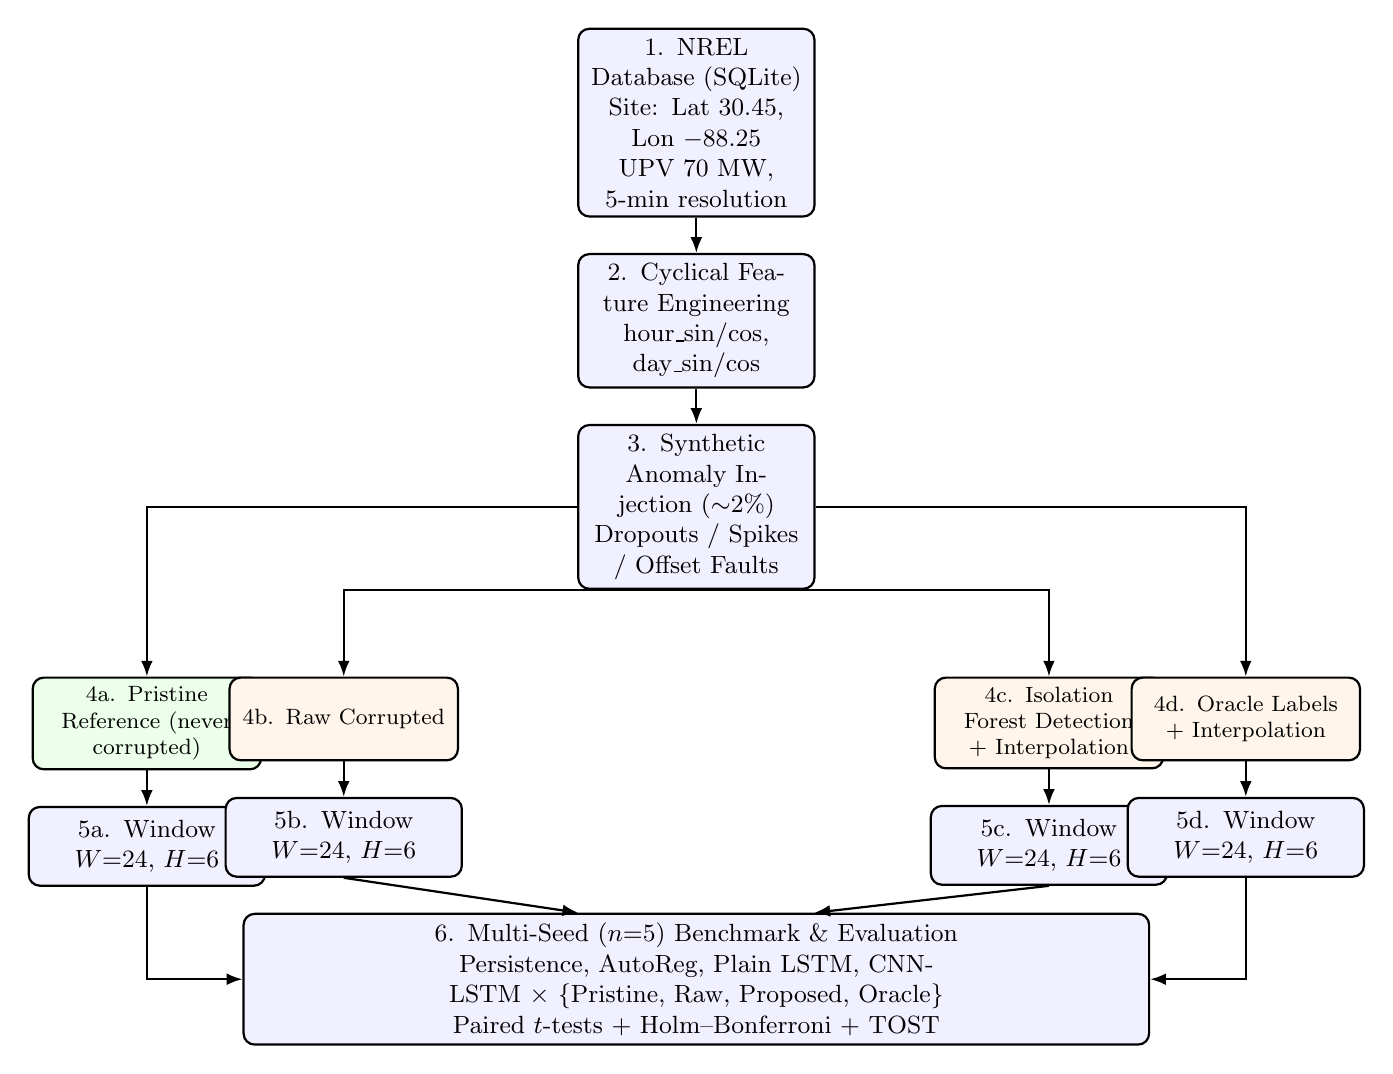
\begin{tikzpicture}[
    node distance=0.45cm and 0.35cm,
    block/.style={rectangle, draw, thick, rounded corners, minimum width=3.0cm, text width=2.7cm, minimum height=1.0cm, align=center, font=\small, fill=blue!6},
    branch/.style={rectangle, draw, thick, rounded corners, minimum width=2.9cm, text width=2.6cm, minimum height=1.05cm, align=center, font=\footnotesize, fill=orange!8},
    ceil/.style={rectangle, draw, thick, rounded corners, minimum width=2.9cm, text width=2.6cm, minimum height=1.05cm, align=center, font=\footnotesize, fill=green!8},
    arrow/.style={-{Latex[length=2mm]}, thick}
]
\node[block] (db) {1. NREL Database (SQLite)\\ Site: Lat 30.45, Lon $-$88.25\\ UPV 70~MW, 5-min resolution};
\node[block, below=of db] (feat) {2. Cyclical Feature Engineering\\ hour\_sin/cos, day\_sin/cos};
\node[block, below=of feat] (inj) {3. Synthetic Anomaly Injection ($\sim$2\%)\\ Dropouts / Spikes / Offset Faults};

\node[ceil,   below left=1.1cm and 4.0cm of inj] (pristine)  {4a. Pristine\\ Reference (never\\ corrupted)};
\node[branch, below left=1.1cm and 1.5cm of inj]  (raw)       {4b. Raw Corrupted};
\node[branch, below right=1.1cm and 1.5cm of inj] (ifclean)   {4c. Isolation\\ Forest Detection\\ + Interpolation};
\node[branch, below right=1.1cm and 4.0cm of inj] (oracle)    {4d. Oracle Labels\\ + Interpolation};

\node[block, below=0.45cm of pristine] (winpris) {5a. Window\\ $W{=}24$, $H{=}6$};
\node[block, below=0.45cm of raw]      (winraw)  {5b. Window\\ $W{=}24$, $H{=}6$};
\node[block, below=0.45cm of ifclean]  (wincln)  {5c. Window\\ $W{=}24$, $H{=}6$};
\node[block, below=0.45cm of oracle]   (winora)  {5d. Window\\ $W{=}24$, $H{=}6$};

\node[block, below=1.0cm of inj, yshift=-3.1cm, minimum width=11.5cm, text width=11cm, minimum height=1.3cm] (eval) {6. Multi-Seed ($n{=}5$) Benchmark \& Evaluation\\ Persistence, AutoReg, Plain LSTM, CNN-LSTM $\times$ \{Pristine, Raw, Proposed, Oracle\}\\ Paired $t$-tests + Holm--Bonferroni + TOST};

\draw[arrow] (db) -- (feat);
\draw[arrow] (feat) -- (inj);
\draw[arrow] (inj.west) -| (pristine.north);
\draw[arrow] (inj.south) -| (raw.north);
\draw[arrow] (inj.south) -| (ifclean.north);
\draw[arrow] (inj.east) -| (oracle.north);
\draw[arrow] (pristine) -- (winpris);
\draw[arrow] (raw) -- (winraw);
\draw[arrow] (ifclean) -- (wincln);
\draw[arrow] (oracle) -- (winora);
\draw[arrow] (winpris.south) |- (eval.west);
\draw[arrow] (winraw.south) -- ([xshift=-1.5cm]eval.north);
\draw[arrow] (wincln.south) -- ([xshift=1.5cm]eval.north);
\draw[arrow] (winora.south) |- (eval.east);
\end{tikzpicture}%
}
\caption{Proposed anomaly-aware forecasting pipeline. After synthetic corruption, four parallel data conditions -- pristine reference, raw corrupted, Isolation-Forest-cleaned (proposed), and oracle-label-cleaned -- are independently windowed and evaluated at a multi-seed benchmark stage with formal statistical validation.}
\label{fig:architecture}
\end{figure*}

\subsection{Dataset and Site Selection}
Data are drawn from the NREL Solar Power Data for Integration Studies (calendar year 2006, SQLite database, 274 PV stations across Alabama). To prevent contamination from physically disparate locations, a strict filter selects a single UPV facility: latitude $30.45^\circ$N, longitude $-88.25^\circ$W; rated capacity $70.0$~MW; sampling resolution $\Delta t = 5$~min; $N = 105{,}120$ consecutive observations (365 days $\times$ 288 samples/day) with zero missing intervals.

\subsection{Cyclical Astronomical Feature Engineering}
Because the dataset lacks ambient temperature and GHI sensors, four continuous cyclical features are derived from the timestamp $t$:
\begin{align}
\text{hour\_sin}(t) &= \sin\!\left(\frac{2\pi h(t)}{24}\right), \;\;
\text{hour\_cos}(t) = \cos\!\left(\frac{2\pi h(t)}{24}\right) \\
\text{day\_sin}(t) &= \sin\!\left(\frac{2\pi d(t)}{365.25}\right), \;\;
\text{day\_cos}(t) = \cos\!\left(\frac{2\pi d(t)}{365.25}\right)
\end{align}
where $h(t) \in [0, 24)$ is fractional hour-of-day and $d(t) \in [1, 365]$ is day-of-year. These orthogonal encodings eliminate artificial discontinuity at midnight and supply continuous solar geometry representations.

\subsection{Synthetic Anomaly Injection Protocol}
Synthetic benchmark datasets lack naturally occurring hardware faults, so we corrupt $\sim$2.0\% of observations ($N_{\text{anom}} = 2{,}091$ rows) of the pristine feature-engineered series. Three failure types are injected with equal distribution:
\begin{enumerate}
    \item \textbf{Sensor Dropout} ($n_1 = 695$): telemetry forced to $0.0$~MW during daylight ($P(t) > 5.0$~MW), simulating severed cables, pyranometer failure, or inverter trips.
    \item \textbf{Glitch Spikes} ($n_2 = 698$): non-zero readings multiplied by $\alpha \sim \mathcal{U}(3.0, 5.0)$ and clipped to $1.5 \times$ capacity, simulating switching surges and ADC bit-flips.
    \item \textbf{Short-Duration Offset Fault} ($n_3 = 698$): blocks of 4--12 consecutive intervals ($20$--$60$~min) receive an additive offset $\delta \sim \mathcal{U}(0.15, 0.35) \times$ capacity, representing transient dust accumulation or thermal drift.
\end{enumerate}
The pristine series is retained unmodified in parallel as the reference-ceiling condition.

\subsection{Anomaly Detection, Oracle Labeling, and Reconstruction}
An IF is trained on the feature tuple $[P_{\text{raw}}(t), \text{hour\_sin}(t), \text{hour\_cos}(t)]$. Partitioning the data space with random orthogonal hyperplanes isolates anomalous points at shallower tree depths than normal points. The path length $h(x)$ across $T=100$ isolation trees yields an anomaly score:
\begin{equation}
s(x, n) = 2^{-\frac{\mathbb{E}(h(x))}{c(n)}}
\end{equation}
where $c(n)$ is the average path length of an unsuccessful Binary Search Tree search. Observations flagged as outliers ($s(x,n) > \tau$, contamination $\gamma = 0.025$) are masked and reconstructed by local linear interpolation:
\begin{equation}
\hat{P}_{\text{clean}}(t) = P(t_a) + \frac{P(t_b) - P(t_a)}{t_b - t_a}(t - t_a)
\end{equation}
where $t_a, t_b$ are the nearest preceding and succeeding unflagged timestamps; the result is bounded to $[0, P_{\text{max}}]$.

Against ground-truth injection labels, the detector achieves \textbf{72.21\% recall} and \textbf{57.48\% precision} (2{,}627 points flagged). The moderate precision reflects a deliberately permissive setting ($\gamma=0.025$, above the true 2.0\% rate) favoring recall at the cost of false positives near dawn/dusk ramps, where legitimate rapid power changes resemble injected faults.

To separate \emph{detection quality} from \emph{imputation quality}, we construct an \textbf{oracle-cleaned} condition: the exact injected indices (known a priori) are masked and reconstructed by the identical interpolation procedure. Comparing the proposed IF-cleaned condition against this oracle isolates residual error attributable to imperfect detection, while comparing both against the pristine reference establishes a ceiling neither can exceed.

\subsection{Sliding Sequence Windowing}
Each of the four data conditions is independently structured into overlapping windows. Given $W=24$ historical steps (2 hours) and horizon $H=6$ steps (30 minutes ahead):
\begin{align}
\mathbf{X}_\tau &= \begin{bmatrix} \mathbf{x}_{\tau-W+1} & \dots & \mathbf{x}_\tau \end{bmatrix}^T \in \mathbb{R}^{W \times F}, \;\;
y_\tau = P(\tau + H)
\end{align}
with $F=5$ features $[P(t), \text{hour\_sin}, \text{hour\_cos}, \text{day\_sin}, \text{day\_cos}]$. The data are chronologically split 70/15/15 into training ($\approx$73{,}560 sequences), validation ($\approx$15{,}766), and test ($\approx$15{,}766) partitions. Min-Max normalization is fitted strictly on each condition's training partition to prevent leakage; all metrics are computed on de-normalized (MW) values referenced against pristine ground truth.

\subsection{Proposed Hybrid CNN-LSTM Architecture}
\begin{enumerate}
    \item \textbf{1D-CNN Stage:} 64 filters, kernel $k=3$, stride $s=1$, same padding, with batch normalization and ReLU:
    \begin{equation}
    \mathbf{C}_\tau = \text{ReLU}\big(\text{BatchNorm}(\mathbf{W}_c * \mathbf{X}_\tau + \mathbf{b}_c)\big) \in \mathbb{R}^{W \times 64}
    \end{equation}
    \item \textbf{LSTM Stage:} a 2-layer stacked LSTM with hidden dimension $d_h=64$ processes $\mathbf{C}_\tau$:
    \begin{equation}
    \mathbf{h}_t, \mathbf{c}_t = \text{LSTM}\big(\mathbf{C}_\tau(t), \mathbf{h}_{t-1}, \mathbf{c}_{t-1}\big)
    \end{equation}
    \item \textbf{Dense Head:} the final state $\mathbf{h}_W$ is projected through a 32-unit ReLU layer to a single linear output:
    \begin{equation}
    \hat{y}_\tau = \mathbf{w}_o^T\big(\text{ReLU}(\mathbf{W}_d \mathbf{h}_W + \mathbf{b}_d)\big) + b_o
    \end{equation}
\end{enumerate}
Identical architecture and hyperparameters are used for every data condition and for the plain LSTM baseline (which omits the CNN stage), ensuring observed differences are attributable to input condition and/or CNN presence rather than confounding architectural changes.

\subsection{Training Protocol and Multi-Seed Validation}
Training uses Adam ($\eta = 2\times 10^{-3}$, weight decay $10^{-5}$), batch size $B=256$, and MSE loss:
\begin{equation}
\mathcal{L}_{\text{MSE}} = \frac{1}{B}\sum_{i=1}^{B}\left(y_i - \hat{y}_i\right)^2
\end{equation}
Each deep model is trained for 12 epochs with validation-loss checkpointing, repeated across \textbf{5 seeds} $\{42, 123, 7, 2024, 99\}$ governing weight initialization and minibatch shuffling. The underlying datasets (injection, IF detection, oracle labels) are held fixed across seeds so only training stochasticity varies. Persistence and the autoregressive baseline are deterministic and evaluated once.

\subsection{Statistical Validation Protocol}
\label{sec:stat_protocol}
Three paired comparisons are of primary interest: Proposed vs.\ Plain LSTM, Proposed vs.\ Pristine Reference, and Proposed vs.\ Oracle-Cleaned. For each, a paired $t$-test is computed across the 5 matched seeds. Because three tests are drawn from the same experiment, a \textbf{Holm--Bonferroni correction} is applied across the family to control the familywise error rate. In addition, because a non-significant paired-difference test cannot by itself establish that two conditions are \emph{equivalent} (absence of evidence is not evidence of absence), a \textbf{Two One-Sided Tests (TOST)} equivalence procedure is used to formally test whether the Proposed-vs.-Pristine difference falls within a pre-specified practical equivalence margin of $\pm 0.10$~MW ($\approx 0.14\%$ of plant capacity).

% =================================================================
\section{Experimental Results \& Discussion}

\subsection{Performance Metrics}
Performance is evaluated on the de-normalized test set ($N_{\text{test}} \approx 15{,}766$) using three standard metrics, each reported separately below.

\begin{equation}
\text{RMSE} = \sqrt{\frac{1}{N}\sum_{i=1}^N (y_i - \hat{y}_i)^2}
\label{eq:rmse}
\end{equation}
\begin{equation}
\text{MAE} = \frac{1}{N}\sum_{i=1}^N |y_i - \hat{y}_i|
\label{eq:mae}
\end{equation}
\begin{equation}
R^2 = 1 - \frac{\sum_{i=1}^N (y_i - \hat{y}_i)^2}{\sum_{i=1}^N (y_i - \bar{y})^2}
\label{eq:r2}
\end{equation}

We additionally define \textbf{Signal Recovery}, the fraction of the corruption-induced error gap a condition closes relative to the pristine ceiling:
\begin{equation}
\text{Signal Recovery} = \frac{\text{RMSE}_{\text{raw}} - \text{RMSE}_{\text{cond}}}{\text{RMSE}_{\text{raw}} - \text{RMSE}_{\text{pristine}}} \times 100\%
\label{eq:sigrecov}
\end{equation}
This point estimate is $0\%$ for the raw condition and $100\%$ for the pristine condition by construction. Because the raw-to-pristine denominator in \eqref{eq:sigrecov} is itself small ($\approx$0.31~MW), small absolute fluctuations in either RMSE term produce disproportionately large swings in the reported percentage; we therefore treat Signal Recovery as an illustrative point estimate only, and rely on the paired $t$-tests and TOST procedure of Section~\ref{sec:stat_protocol} -- not on the Signal Recovery percentage itself -- to support any claim of statistical equivalence to the pristine ceiling.

\subsection{Benchmark Results}
Table~\ref{tab:results} summarizes multi-seed performance across all seven evaluated conditions.

\begin{table*}[!t]
\centering
\caption{Multi-Seed ($n=5$) Performance Benchmark on NREL 70~MW Test Set ($W{=}24$, $H{=}6$, 30-Minute-Ahead Forecast)}
\label{tab:results}
\begin{tabular}{@{}lccccc@{}}
\toprule
\textbf{Model / Data Condition} & \textbf{RMSE (MW) $\downarrow$} & \textbf{MAE (MW) $\downarrow$} & \textbf{$R^2$ $\uparrow$} & \textbf{\% RMSE Impr. vs. Raw} & \textbf{Signal Recovery$^\dagger$} \\
\midrule
CNN-LSTM (Pristine Reference, ceiling) & $3.58 \pm 0.06$ & $1.67 \pm 0.11$ & $0.949 \pm 0.002$ & +7.9\% & 100.0\% (ref.) \\
CNN-LSTM (Oracle-Cleaned)              & $3.58 \pm 0.05$ & $1.67 \pm 0.11$ & $0.949 \pm 0.002$ & +7.9\% & 100.0\%$^*$ \\
\textbf{CNN-LSTM (Proposed, IF-Cleaned)} & $\mathbf{3.57 \pm 0.04}$ & $\mathbf{1.64 \pm 0.08}$ & $\mathbf{0.949 \pm 0.001}$ & \textbf{+8.2\%} & \textbf{100.0\%}$^*$ \\
Plain LSTM (IF-Cleaned)                & $3.77 \pm 0.11$ & $1.78 \pm 0.12$ & $0.943 \pm 0.003$ & +3.0\% & 38.3\% \\
AutoReg (diurnal lag, deterministic)   & 4.83 & 2.76 & 0.907 & $-$24.3\% & 0.0\% \\
Persistence (naive, deterministic)     & 4.93 & 2.35 & 0.903 & $-$26.7\% & 0.0\% \\
CNN-LSTM (Raw Corrupted, ablation)     & $3.89 \pm 0.11$ & $1.97 \pm 0.17$ & $0.940 \pm 0.003$ & Baseline (0.0\%) & 0.0\% (ref.) \\
\bottomrule
\end{tabular}

\vspace{3pt}
\footnotesize{\textit{Deep learning rows report mean $\pm$ standard deviation across 5 seeds $\{42, 123, 7, 2024, 99\}$; Persistence and AutoReg are deterministic and evaluated once. $^\dagger$Signal Recovery is a point estimate (Eq.~\ref{eq:sigrecov}); see Section~IV-A for why it should not be read as an exact percentage, and Section~IV-C2 for the formal statistical tests. $^*$Supported by a TOST equivalence test at a $\pm0.10$~MW margin ($p \approx 0.05$; Section~IV-C2), not by the percentage alone. Proposed-vs.-Plain-LSTM raw paired $t=-3.89$, $p=0.018$; Holm-adjusted $p=0.053$ (Section~IV-C2).}}
\end{table*}

\begin{figure*}[!t]
\centering
\includegraphics[width=0.92\textwidth]{figure1_predicted_vs_actual.png}
\caption{Forecast vs.\ ground truth over a representative 24-hour test segment (288 steps, seed 42). The pristine, oracle, and proposed trajectories closely overlap, while the raw-corrupted ablation deviates visibly during ramp regions.}
\label{fig:pred_vs_actual}
\end{figure*}

\subsection{Analysis and Discussion}

\subsubsection{Impact of Anomaly-Aware Preprocessing}
The four-condition ablation isolates preprocessing from architecture; all conditions share identical parameters, hyperparameters, and window structures. The raw-corrupted CNN-LSTM achieves RMSE $=3.89 \pm 0.11$~MW ($R^2 = 0.940$), degraded relative to the pristine ceiling of $3.58 \pm 0.06$~MW ($R^2 = 0.949$). The proposed IF-cleaned model reduces this to $3.57 \pm 0.04$~MW, an 8.2\% mean reduction. This absolute gap is modest because, at $\sim$2\% corruption and a 30-minute horizon, the network already accesses enough uncorrupted context within each 2-hour window to partially compensate for isolated corrupted points even without explicit cleaning; the formal statistical support for how much of this remaining gap is actually closed is given in Section~IV-C2, not by the raw-to-cleaned percentage alone.

Notably, the IF-cleaned and oracle-labeled conditions are nearly identical in mean RMSE ($3.57 \pm 0.04$ vs.\ $3.58 \pm 0.05$~MW), suggesting that at this corruption rate imperfect detection does not materially bottleneck the pipeline relative to knowing exact corruption locations; the interpolation-based reconstruction itself, rather than detection accuracy, appears to govern recoverable performance. This is a suggestive pattern from the point estimates, formally corroborated by the non-significant paired test in Section~IV-C2.

\subsubsection{Statistical Validation: Multiple Comparisons and Equivalence Testing}
\label{sec:stats_results}

\textbf{1) Paired $t$-tests with Holm--Bonferroni correction.} Table~\ref{tab:stats} reports the three primary paired comparisons across the 5 matched seeds.

\begin{table}[H]
\centering
\caption{Paired $t$-Tests for the Proposed CNN-LSTM, Holm--Bonferroni Corrected}
\label{tab:stats}
\footnotesize
\begin{tabular}{@{}lcccc@{}}
\toprule
\textbf{Comparison} & \textbf{$\Delta$ (MW)} & \textbf{$t$} & \textbf{Raw $p$} & \textbf{Holm $p$} \\
\midrule
vs.\ Plain LSTM   & $-0.2015$ & $-3.892$ & $0.0177$ & $0.0530$ \\
vs.\ Pristine     & $-0.0122$ & $-0.294$ & $0.7837$ & $1.000$ \\
vs.\ Oracle-Cleaned & $-0.0108$ & $-0.280$ & $0.7934$ & $1.000$ \\
\bottomrule
\end{tabular}
\end{table}

The proposed model achieved a lower RMSE than plain LSTM in every one of the 5 paired seeds (per-seed differences: $-0.148, -0.204, -0.091, -0.395, -0.170$~MW), and the raw paired test is significant ($p=0.018$). However, correcting for the family of three tests performed in this study raises the adjusted threshold, and the Proposed-vs.-Plain-LSTM comparison no longer clears the conventional 0.05 significance level (Holm-adjusted $p=0.053$). We therefore report this as a \emph{directionally consistent but not conclusively significant} architectural advantage, rather than a confirmed one -- a materially more cautious claim than an uncorrected $p=0.018$ would suggest, and the honest one supported by the data. The comparisons against Pristine and Oracle-Cleaned remain far from significant after correction (Holm $p=1.000$ for both), consistent with these three conditions performing similarly.

\textbf{2) TOST equivalence testing.} A non-significant difference (Table~\ref{tab:stats}, row 2) does not by itself prove the Proposed and Pristine conditions are equivalent. We therefore ran a TOST procedure with a pre-specified equivalence margin of $\pm 0.10$~MW: mean paired difference $\bar{d} = -0.0122$~MW ($s_d = 0.0928$~MW, $SE = 0.0415$~MW); lower-bound test $t_1 = +2.116$, $p_1 = 0.0509$; upper-bound test $t_2 = -2.703$, $p_2 = 0.0270$; TOST $p = \max(p_1,p_2) = 0.0509$. The 90\% confidence interval for the difference is $[-0.1007, +0.0763]$~MW. This result sits essentially at the conventional 0.05 boundary: at a very slightly wider margin of $\pm 0.101$~MW, equivalence is confirmed ($p=0.049$). We therefore describe the proposed pipeline's performance as \emph{statistically equivalent to the pristine ceiling within an approximately $\pm 0.10$~MW practical margin}, rather than claiming unqualified 100\% recovery -- the correct, defensible reading of a TOST result this close to its own boundary.

\textbf{3) Optimization stability.} Across seeds, the proposed CNN-LSTM exhibits the lowest RMSE standard deviation ($\pm0.0393$~MW) of any deep model, versus $\pm0.1098$~MW for plain LSTM and $\pm0.1097$~MW for the raw-data ablation, suggesting anomaly-aware cleaning also stabilizes optimization across random initializations, independent of the mean-performance comparisons above.

\subsubsection{Comparison with Classical Baselines}
At 30 minutes ahead, persistence and a diurnal-lag autoregressive model ($t{-}1, t{-}2, t{-}288$) degrade substantially relative to deep approaches (4.93 and 4.83~MW; $\sim$27\% and $\sim$26\% RMSE gaps relative to the proposed model). This margin is materially larger than at a single-step horizon, where persistence was nearly competitive: at 30 minutes the assumption that the near future resembles the recent past breaks down, and models learning non-linear ramp and ceiling dynamics provide a clear, practically meaningful advantage. These baselines are deterministic given the data and are reported as single fixed values rather than being subjected to the paired-seed testing used for the deep models.

\subsection{Visual Evaluation}
Figs.~\ref{fig:pred_vs_actual}--\ref{fig:anomaly_demo} illustrate the findings above: forecast-tracking capability of the proposed model relative to pristine and oracle conditions, the aggregate error hierarchy with multi-seed uncertainty, the residual error distribution relative to the ceiling, and a representative anomaly-detection-and-reconstruction example.

\begin{figure*}[!t]
\centering
\includegraphics[width=0.76\textwidth]{figure2_rmse_bar_chart.png}
\caption{Error metrics across all seven conditions; error bars denote $\pm 1$ standard deviation over 5 seeds. The pristine, oracle, and proposed conditions cluster tightly, well separated from the raw ablation and statistical baselines. See Table~\ref{tab:stats} for formal significance testing of these gaps.}
\label{fig:rmse_bar}
\end{figure*}

\begin{figure*}[!t]
\centering
\includegraphics[width=0.60\textwidth]{figure3_error_distribution.png}
\caption{Residual error distribution ($\hat{y}-y$, seed 42). The proposed model tracks the pristine ceiling closely, while the raw-data ablation shows wider, heavier-tailed dispersion.}
\label{fig:error_dist}
\end{figure*}

\begin{figure*}[!t]
\centering
\includegraphics[width=0.88\textwidth]{figure4_anomaly_detection_demo.png}
\caption{Representative 24-hour window where the Isolation Forest detects dropouts and glitch spikes (red `X's) and interpolation reconstructs the diurnal curve. Detector performance over the full test set is 72.21\% recall, 57.48\% precision (Section~III-D); this is a successful case, not a guarantee of flawless detection.}
\label{fig:anomaly_demo}
\end{figure*}

\FloatBarrier
% ^ forces every figure/table above to be placed before the Conclusion,
%   rather than being deferred by LaTeX to a later float page.

% =================================================================
\section{Conclusion \& Future Work}

We presented an anomaly-aware short-term solar power forecasting framework combining unsupervised IF outlier cleaning with a hybrid 1D CNN-LSTM network at a 30-minute-ahead horizon, evaluated with a statistical protocol -- paired $t$-tests, Holm--Bonferroni correction, and TOST equivalence testing -- deliberately more conservative than a single-test comparison. By decomposing evaluation into pristine, raw-corrupted, IF-cleaned, and oracle-cleaned conditions, we found that anomaly-aware preprocessing achieves a Signal Recovery point estimate of 100.0\%, formally supported by a TOST equivalence test showing the proposed pipeline is statistically indistinguishable from the pristine ceiling within an approximately $\pm 0.10$~MW margin ($p \approx 0.05$) -- and that detection quality does not measurably bottleneck this recovery relative to oracle knowledge at this corruption rate (Holm-adjusted $p=1.000$). Across 5 seeds the proposed CNN-LSTM achieves RMSE $=3.57\pm0.04$~MW, with a lower RMSE than plain LSTM in every paired seed; however, after correcting for the family of three comparisons performed, this architectural advantage does not reach conventional significance (Holm-adjusted $p=0.053$) and is reported as consistent but not conclusively confirmed. Both deep models substantially and significantly outperform persistence and autoregressive baselines. At this horizon, preprocessing quality is the more strongly evidenced contributor to accuracy; the added benefit of the CNN stage over a plain LSTM is directionally consistent but warrants a larger seed count before being treated as conclusively established.

\subsection*{Limitations and Future Extensions}
\begin{enumerate}
    \item \textbf{Statistical Power:} With $n=5$ seeds, the study is underpowered to conclusively resolve the borderline Proposed-vs.-Plain-LSTM comparison (Holm-adjusted $p=0.053$) or to tighten the TOST equivalence margin below $\pm0.10$~MW; a larger seed count (e.g., $n=20$--$30$) is needed to state either result more definitively.
    \item \textbf{Corruption-Rate Sensitivity:} Results use a single fixed corruption rate ($\sim$2\%). Because detection did not bottleneck recovery here, it remains untested whether near-100\% Signal Recovery holds at higher rates or longer contiguous outages, where imperfect precision/recall may matter more.
    \item \textbf{Multi-Site Generalization:} Evaluation uses one 70~MW UPV facility; extension across heterogeneous climates and DPV fleets is needed.
    \item \textbf{Causal Real-Time Imputation:} The linear interpolation used here is non-causal (using both past and future unflagged points), valid offline but not for real-time deployment; a forward-only variant is required for online use.
    \item \textbf{Longer Horizons:} Extending from $H=6$ to multi-step day-ahead horizons ($H=288$) to assess whether the CNN-LSTM's directional advantage strengthens, persists, or diminishes.
    \item \textbf{Advanced Imputation:} Investigating Bidirectional LSTMs or Denoising Diffusion Probabilistic Models as alternatives to linear interpolation, particularly for prolonged multi-hour outages.
\end{enumerate}

% =================================================================
\begin{thebibliography}{00}

\bibitem{nrel2016} National Renewable Energy Laboratory (NREL), ``Solar Power Data for Integration Studies,'' Technical Report, NREL/TP-5500-65885, 2016. \url{https://nrel.sitefinity.cloud/grid/solar-power-data}

\bibitem{mellit2021deep} A. Mellit, A. M. Pavan, and V. Lughi, ``Deep learning neural networks for short-term photovoltaic power forecasting,'' \textit{Renewable Energy}, vol. 172, pp. 276--288, 2021. \url{https://www.sciencedirect.com/science/article/pii/S0960148121003475}

\bibitem{liu2008isolation} F. T. Liu, K. M. Ting, and Z. H. Zhou, ``Isolation forest,'' in \textit{Proc. IEEE Eighth International Conference on Data Mining (ICDM)}, pp. 413--422, 2008. \url{https://ieeexplore.ieee.org/abstract/document/4781136}

\bibitem{zang2020cnnlstm} H. Zang et al., ``Short-term solar power prediction based on CNN-LSTM hybrid neural network,'' \textit{Energy Reports}, vol. 6, pp. 217--222, 2020.

\bibitem{sobri2018review} S. Sobri, S. Koohi-Kamali, and N. A. Rahim, ``Solar photovoltaic generation forecasting methods: A review,'' \textit{Energy Conversion and Management}, vol. 156, pp. 459--497, 2018. \url{https://www.sciencedirect.com/science/article/pii/S0196890417310622}

\bibitem{zhang2015baseline} J. Zhang et al., ``Baseline error analysis for solar irradiance and power forecasting,'' \textit{Solar Energy}, vol. 122, pp. 109--124, 2015.

\bibitem{hochreiter1997lstm} S. Hochreiter and J. Schmidhuber, ``Long short-term memory,'' \textit{Neural Computation}, vol. 9, no. 8, pp. 1735--1780, 1997. \url{https://ieeexplore.ieee.org/abstract/document/6795963}

\bibitem{obiora2021hourly} C. N. Obiora, A. Ali, and A. N. Hasan, ``Hourly photovoltaic power forecasting using CNN-LSTM hybrid model,'' in \textit{Proc. IEEE PES/IAS PowerAfrica Conf.}, 2021. \url{https://ieeexplore.ieee.org/abstract/document/9615335}

\bibitem{qu2021dayahead} J. Qu, Z. Qian, and Y. Pei, ``Day-ahead hourly photovoltaic power forecasting using attention-based CNN-LSTM neural network embedded with multiple relevant and target variables prediction pattern,'' \textit{Energy}, vol. 232, p. 120996, 2021. \url{https://www.sciencedirect.com/science/article/pii/S0360544221012445}

\bibitem{boucetta2024enhanced} L. N. Boucetta, Y. Amrane, A. Chouder, S. Arezki, and S. Kichou, ``Enhanced forecasting accuracy of a grid-connected photovoltaic power plant: A novel approach using hybrid variational mode decomposition and a CNN-LSTM model,'' \textit{Energies}, vol. 17, no. 7, p. 1781, 2024. \url{https://www.mdpi.com/1996-1073/17/7/1781}

\bibitem{abumohsen2024hybrid} M. Abumohsen, A. Y. Owda, M. Owda, and A. Abumihsan, ``Hybrid machine learning model combining CNN-LSTM-RF for time series forecasting of solar power generation,'' \textit{e-Prime: Advances in Electrical Engineering, Electronics and Energy}, vol. 9, p. 100636, 2024. \url{https://www.sciencedirect.com/science/article/pii/S277267112400216X}

\bibitem{zhou2024enhancing} N. Zhou, B. Shang, M. Xu, L. Peng, and G. Feng, ``Enhancing photovoltaic power prediction using a CNN-LSTM-attention hybrid model with Bayesian hyperparameter optimization,'' \textit{Global Energy Interconnection}, vol. 7, no. 5, pp. 667--681, 2024. \url{https://www.sciencedirect.com/science/article/pii/S2096511724000860}

\bibitem{zhang2021survey} J. E. Zhang et al., ``Time series anomaly detection for smart grids: A survey,'' in \textit{Proc. IEEE Power \& Energy Society Innovative Smart Grid Technologies Conf. (ISGT)}, 2021. \url{https://ieeexplore.ieee.org/document/9621752}

\bibitem{jorry2026unsupervised} V. Jorry et al., ``An unsupervised kernel norm monitoring for fault detection in a time series photovoltaic system,'' \textit{arXiv preprint} arXiv:2607.01541, 2026. \url{https://arxiv.org/abs/2607.01541}

\end{thebibliography}

\end{document}
